% !TeX program = pdflatex
% Main document: main.tex (keep at the project root).
\documentclass[11pt]{article}
\usepackage[review]{acl}
\usepackage{times}
\usepackage{latexsym}
\usepackage[T1]{fontenc}
\usepackage[utf8]{inputenc}
\usepackage{microtype}
\usepackage{amsmath,amssymb}
\usepackage{booktabs,tabularx,array}
\usepackage{graphicx}
\usepackage{tikz}
\usetikzlibrary{arrows.meta,positioning,fit,calc}
\usepackage{algorithm}
\usepackage{algpseudocode}
\newcommand{\method}{\mbox{\textsc{JIT-Compose}}}
\newcommand{\state}{\mathcal{S}}
\newcommand{\rub}{\widehat{\mathcal{R}}}
\newcommand{\crit}{\mathcal{C}}
\newcommand{\team}{\mathcal{T}}
\newcommand{\trace}{\mathcal{Z}}
\newcommand{\ind}{\mathbf{1}}
\newcommand{\na}{\textemdash}
\hypersetup{pdftitle={JIT-Compose: Evolving Multi-Agent Workflow Synthesis for Open-Ended Generation},pdfauthor={Anonymous},pdfsubject={Working manuscript v3; task-specific workflow synthesis and experience evolution; empirical results not supplied}}

\title{JIT-Compose: Evolving Multi-Agent Workflow Synthesis\\for Open-Ended Generation}
\author{Anonymous Authors}
\date{}
\begin{document}
\maketitle

\begin{abstract}
Open-ended generation requires deciding not only what to write, but how agents should collaborate to produce it. When quality requirements are only partially specified, the central challenge is to anticipate what good work demands and turn those expectations into a suitable writing process. We introduce \method, an experience-driven framework that synthesizes an executable, task-specific multi-agent writing workflow on demand. Predicted rubrics serve both as a specification for workflow construction and as a reference for improving future construction. Before execution, global--local planning refines the requirements and their importance, negotiates agent responsibilities and information dependencies, and instantiates the resulting design as roles, interactions, and verification stages. After submission, independent criterion-level feedback is aligned with the frozen predictions and examined against global coordination records and agent-local trajectories. This supports targeted revisions to requirement prediction, team organization, or execution, rather than an undifferentiated instruction to improve the answer. After attribution, a scoped, structurally valid revision is written directly to versioned reusable experience; no accept, hold, or reject quality-selection stage intervenes. Model parameters and the evaluator remain fixed, while committed experience changes how subsequent teams and workflows are generated. \method\ thus couples just-in-time task adaptation with cross-task evolution: it retains knowledge for constructing the next writing process, not a single process that every task must reuse.
\end{abstract}

\noindent\textbf{Working draft.} Methods follow the supplied system design; empirical results and implementation artifacts have not been supplied for audit. Unfilled tables and diagnostic protocols below are not reported findings.

\section{Introduction}
\label{sec:intro}

A writing system must decide not only what to say, but how the work leading to that response should be organized. Which information should be gathered in parallel? Which conclusions require cross-source checks? Who should reconcile incompatible evidence before drafting? We study how to construct this process for the task at hand, and how feedback from completed tasks should change the construction of the next one.

Consider a report comparing two document-retrieval methods. One agent summarizes each method and a third combines the summaries. Both summaries may be accurate, yet the report can compare measurements obtained on incompatible corpora or workloads. Every agent has completed its assignment, but a critical operation is missing between them: collecting the conditions from both branches and checking whether the comparison is warranted. The remedy is not necessarily another writer or a longer instruction. It may be a different writing workflow.

This illustrative case exposes a \emph{quality-to-coordination gap}: recognizing what good work requires does not ensure that the division of labor can produce it. In open-ended research generation, fine-grained rubrics assess evidence and analytical quality across multiple defensible responses \citep{sharma2025researchrubrics}. In our setting, evaluator-private criteria arrive only after submission. A system must therefore anticipate useful requirements before organizing the work, then interpret the feedback without rewriting its earlier expectations.

\begin{figure*}[t]
\centering
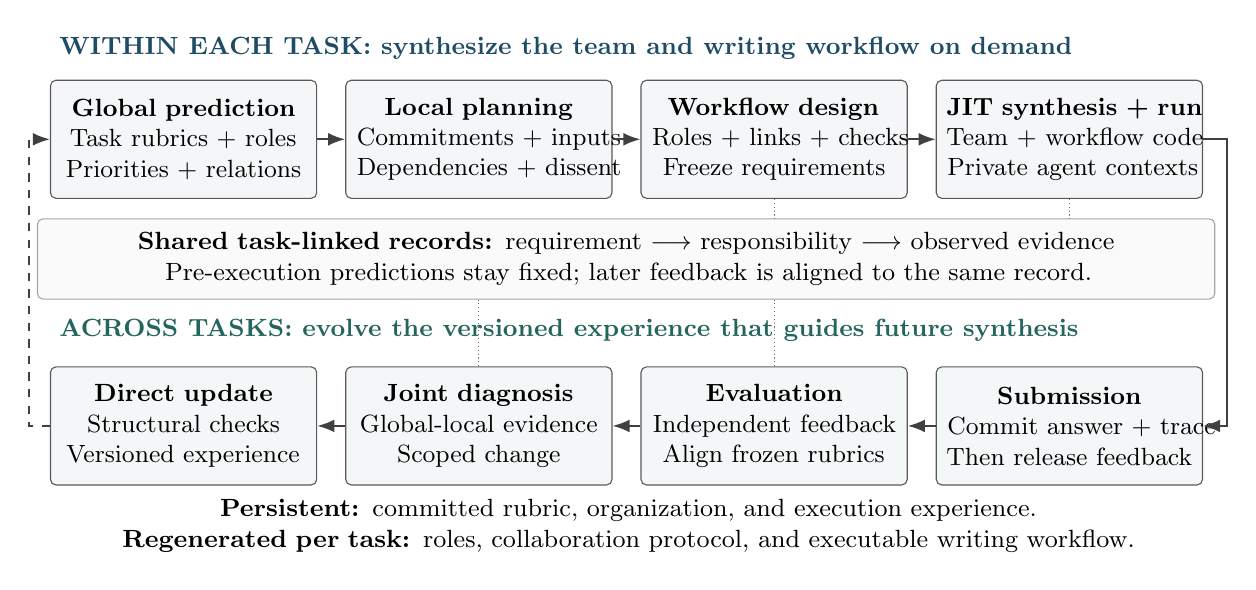
\begin{tikzpicture}[x=1cm,y=1cm,>=Latex,
  box/.style={draw=black!65,rounded corners=2pt,align=center,inner sep=4pt,font=\fontsize{9}{11}\selectfont,minimum height=1.50cm,text width=3.1cm},
  flow/.style={->,line width=.7pt,draw=black!75},
  smallnote/.style={font=\fontsize{9}{11}\selectfont,align=center}]
\definecolor{coordblue}{RGB}{31,76,101}
\definecolor{evolveteal}{RGB}{36,102,93}
\node[anchor=west,font=\small\bfseries,text=coordblue] at (0,1.16) {WITHIN EACH TASK: synthesize the team and writing workflow on demand};
\node[box,fill=coordblue!5] (g) at (1.7,0) {\mbox{\textbf{Global prediction}}\\\mbox{Task rubrics + roles}\\\mbox{Priorities + relations}};
\node[box,fill=coordblue!5] (l) at (5.45,0) {\mbox{\textbf{Local planning}}\\\mbox{Commitments + inputs}\\\mbox{Dependencies + dissent}};
\node[box,fill=coordblue!5] (c) at (9.2,0) {\mbox{\textbf{Workflow design}}\\\mbox{Roles + links + checks}\\\mbox{Freeze requirements}};
\node[box,fill=coordblue!5] (e) at (12.95,0) {\mbox{\textbf{JIT synthesis + run}}\\\mbox{Team + workflow code}\\\mbox{Private agent contexts}};
\draw[flow] (g)--(l); \draw[flow] (l)--(c); \draw[flow] (c)--(e);
\node[draw=black!35,fill=black!2,rounded corners=2pt,text width=14.6cm,align=center,font=\fontsize{9}{11}\selectfont,inner sep=5pt] (link) at (7.32,-1.52) {\textbf{Shared task-linked records:} requirement $\longrightarrow$ responsibility $\longrightarrow$ observed evidence\\Pre-execution predictions stay fixed; later feedback is aligned to the same record.};
\draw[densely dotted,draw=black!55] (c.south) -- (c.south |- link.north);
\draw[densely dotted,draw=black!55] (e.south) -- (e.south |- link.north);
\node[anchor=west,font=\small\bfseries,text=evolveteal] at (0,-2.42) {ACROSS TASKS: evolve the versioned experience that guides future synthesis};
\node[box,fill=evolveteal!5] (v) at (1.7,-3.64) {\mbox{\textbf{Direct update}}\\\mbox{Structural checks}\\\mbox{Versioned experience}};
\node[box,fill=evolveteal!5] (d) at (5.45,-3.64) {\mbox{\textbf{Joint diagnosis}}\\\mbox{Global-local evidence}\\\mbox{Scoped change}};
\node[box,fill=evolveteal!5] (j) at (9.2,-3.64) {\mbox{\textbf{Evaluation}}\\\mbox{Independent feedback}\\\mbox{Align frozen rubrics}};
\node[box,fill=evolveteal!5] (a) at (12.95,-3.64) {\mbox{\textbf{Submission}}\\\mbox{Commit answer + trace}\\\mbox{Then release feedback}};
\draw[flow] (a)--(j); \draw[flow] (j)--(d); \draw[flow] (d)--(v);
\draw[flow] (e.east)--++(.30,0)|-(a.east);
\draw[flow,dashed] (v.west)--++(-.27,0)|-(g.west);
\draw[densely dotted,draw=black!55] (d.north) -- (d.north |- link.south);
\draw[densely dotted,draw=black!55] (j.north) -- (j.north |- link.south);
\node[smallnote,text width=14.7cm] at (7.32,-4.91) {\textbf{Persistent:} committed rubric, organization, and execution experience.\\\textbf{Regenerated per task:} roles, collaboration protocol, and executable writing workflow.};
\end{tikzpicture}
\caption{\method\ operates on two timescales. For the current task, anticipated quality requirements and local plans condition an executable team and writing workflow. After submission, the frozen expectations and execution evidence support scoped lessons, directly persisted after structural and provenance checks without a quality-promotion gate. The dashed return carries versioned experience to later requests, not a fixed team. Model weights and the evaluator remain frozen. Arrows indicate process or record linkage, not causal effects.}
\label{fig:overview}
\end{figure*}


We introduce \method, short for \emph{Just-in-Time Composition of Agent Teams and Workflows}. Given a new problem, it predicts task-specific quality requirements, negotiates responsibilities through global--local planning, and synthesizes an executable multi-agent writing workflow. Here, a workflow specifies roles, information dependencies, tool use, verification, and final synthesis---not merely an outline or prose style. The same system can construct a new organization for each task rather than require every task to reuse one fixed process.

The framework operates on two timescales. \emph{Within a task}, predicted rubrics supply a provisional specification for team and workflow synthesis. A global analyzer identifies priorities and candidate roles; local plans expose missing inputs, conflicting assumptions, and capability limits; reconciliation turns these constraints into an executable design. \emph{Across tasks}, criterion-level feedback is aligned with the frozen predictions and distributed execution records. The system distinguishes what it failed to anticipate, what the organization failed to support, and what execution failed to deliver, then proposes changes to the corresponding experience. Attributed changes directly update the versioned experience used for subsequent workflows; model parameters and the evaluator remain fixed.

Predicted requirements connect these timescales. Before execution, they link a quality expectation to accepted responsibilities and expected evidence. After submission, the same links route feedback to the relevant plans, interactions, and local traces. The question is not simply ``which agent failed?'' but \emph{what was expected, how was it assigned, and what happened?} Different histories behind the same low score can warrant different lessons for future synthesis. The resulting lesson changes future workflow construction rather than rewriting the already-submitted answer; whether it improves later tasks is a separate empirical question.

Task-conditioned harness generation is inherited from JIT-Agent \citep{zhang2026jit}; evolving orchestration skills, collaborative reflection, and prospective rubric guidance have close precedents in Skill-MAS, Meta-Team, and Think-with-Rubrics \citep{lin2026skillmas,hao2026metateam,yu2026thinkrubrics}. Our focus is the quality-linked synthesis-and-update procedure connecting these decisions. Neither on-demand generation nor an evolving builder is claimed in isolation. The central question is whether using predicted requirements to shape executable collaboration, and feedback to revise that shaping process, adds value beyond supplying the same requirements as answer guidance.

The paper develops three methodological contributions: quality-conditioned synthesis of task-specific agent teams and writing workflows; global--local, evidence-linked updates to the experience used for subsequent synthesis; and controlled tests that distinguish organizational use, update utility, and frozen-state transfer. The tests also separate anticipating an information need from guessing an answer-bearing criterion. Together they examine one proposition: \emph{construct the writing process for the current task, and retain evidence-linked knowledge for constructing the next.}

\section{Generated Workflows and Evolving State}
\label{sec:setting}

A task provides a public request $x_t$, permitted tools $\mathcal U_t$, and a resource envelope $B_t$. The independent evaluator holds criteria $\crit_t=\{(c_j,w_j)\}_{j=1}^{m_t}$ and any private reference material. The team cannot access these records before committing its response $y_t$. Public instructions remain available; \emph{open-ended} denotes multiple possible valid responses, not an absence of evaluable requirements.

A generated writing workflow is denoted $\omega_t=(\team_t,h_t)$: $\team_t$ specifies the participating roles and their collaboration, while $h_t$ implements that organization as executable code. It governs evidence gathering, analysis, verification, and final synthesis. This notation combines existing team and harness records; it does not introduce an additional learned module.

The versioned experience state is
\begin{equation}
\state_t=(E_t^R,E_t^O,E_t^X,V_t),
\end{equation}
where the stores contain rubric, organization, and execution experience, and $V_t$ identifies policy and prompt versions. Retrieval excludes the current task, restricted evaluation records, and future experience. With $\theta$ denoting the fixed parameters of the configured generator, analyzers, and executors, one task proceeds as
\begin{align}
(\rub_t,\team_t)&=\operatorname{Build}_{\theta}(x_t,\state_t,B_t),\label{eq:build}\\
h_t&=\operatorname{JIT}_{\theta}(x_t,\rub_t,\team_t,\mathcal U_t),\label{eq:synth}\\
(y_t,\trace_t)&=\operatorname{Run}_{\theta}(h_t,x_t,\mathcal U_t,B_t),\label{eq:run}\\
f_t&=\operatorname{Eval}_{\phi}(x_t,y_t,\crit_t).\label{eq:eval}
\end{align}
Here $\phi$ is a fixed evaluator configuration, not an assumption of unbiased judgment. After an evolution task, a direct attributed update may change $\state_t$; in frozen evaluation it cannot. In both settings, Equations~\ref{eq:build}--\ref{eq:synth} construct a task-specific team and executable workflow. What persists across tasks is $\state_t$, not a mandatory shared $\omega_t$. Learning refers to versioned changes in retrieved experience and policies, not parameter training. Similar tasks may yield similar workflows; novelty of the generated structure is not itself an objective.

The goal is held-out response quality under an explicit resource constraint. Planning, code generation and repair, communication, and synthesis all count toward inference cost. External evaluation, diagnosis, and experience writes are additional measured costs; there are no paired-validation calls in the update path. They cannot be omitted when assessing the value of evolution.

\section{JIT-Compose: Synthesis and Evolution}
\label{sec:method}

\method\ uses predicted rubrics in two directions: as a provisional specification for synthesizing the current workflow, and as a reference for interpreting feedback that may change future synthesis. The connecting records form a requirement--responsibility--evidence graph: anticipated obligation $\rightarrow$ accepted responsibility $\rightarrow$ observed evidence $\rightarrow$ retrospective feedback. This is a view of existing rubric, team, and event records, not a graph-learning algorithm. It preserves why a design decision was made and the evidence relevant to revising it.

\subsection{Predict a Task-Specific Quality Specification}
\label{sec:anticipate}

The global analyzer uses $x_t$ and committed experience to produce initial requirements $\rub_t^g$ and candidate roles. Each predicted item records operational text $d_i$, nonnegative importance $a_i$, confidence $q_i$, expected evidence $e_i$, polarity, provenance, and applicability. Importance is distinct from confidence and from the evaluator's private signed weight $w_j$.

Requirements specify work without inventing its outcome. In the retrieval example, the system can anticipate checking whether measurements use comparable workloads; it need not know those measurements. A relation graph records prerequisite, support, overlap, and trade-off hypotheses. These relationships allow obligations spanning several contributions to influence organization. The graph is not automatically a schedule: semantic relationships can be cyclic even when executable dependencies must be acyclic or explicitly bounded.

General quality priors may seed anticipation, but task-specific evidence expectations must make them actionable. ``Be accurate'' does not specify which comparison must be checked. Predicted obligations can also be wrong or inapplicable, so later feedback can revise their scope rather than merely add more requirements.

\subsection{Co-Design the Team and Its Collaboration}
\label{sec:negotiate}

Each candidate agent receives the public task, relevant predicted requirements, and its proposed capabilities. It returns a local plan: responsibilities it can accept, information it needs, outputs it can produce, collaborators it depends on, and work it cannot cover. It may challenge the global decomposition or add a missing requirement. This exchange is not a vote on whether the initial plan sounds reasonable; it supplies constraints on whether that plan can be carried out.

Global reconciliation produces revised requirements $\rub_t^p$ and
\begin{equation}
\team_t=(\mathcal A_t,C_t,D_t,T_t,b_t),
\end{equation}
representing roles, many-to-many responsibilities, communication and artifact dependencies, tool permissions, and budget allocations. A responsibility links a requirement to an owner or joint owners, required inputs, expected output evidence, a recipient, and a review condition where warranted. The synthesizer is included: information found by a researcher is not yet information used in the final response.

For the running example, local plans may reveal that each researcher can extract measurement conditions but neither can judge cross-source comparability alone. Reconciliation can require a common evidence schema and assign an explicit comparison check before synthesis. The example illustrates the intended mechanism; it is not an observed experimental result.

The coordinator addresses uncovered obligations, redundant work, incompatible assumptions, and resource feasibility. It need not create one agent per rubric, and simple tasks may use one executor. Decisions are model-mediated; deterministic checks enforce schemas, permissions, budgets, and schedulable dependencies, not semantic optimality. Both $\rub_t^g$ and $\rub_t^p$, together with $\team_t$, are frozen as separate pre-execution records. Later feedback cannot retrospectively improve those snapshots.

\subsection{Synthesize and Execute the Writing Workflow}
\label{sec:execution}

Conditioned on the public task, reconciled requirements, and team specification, the JIT synthesizer generates the original five-file harness format: memory, planning, action, tool policy, and prompts. The inherited protocol $h=(M,P,A,F)$ provides the executable substrate \citep{zhang2026jit}. Memory organizes private contexts and shared evidence; the execution-time planning module deterministically reads the already-frozen team directives and dependencies, without another model call; tool policy controls the available capabilities; and action coordinates execution and termination. Together with $\team_t$, these modules instantiate the task's writing workflow $\omega_t$.

Generated modules may call stable MAS primitives, but the participating roles, information handoffs, checks, and synthesis procedure remain conditioned on the current problem. TeamSpec must affect these decisions during actual execution, not merely describe a fixed workflow in its metadata. Protocol and runtime checks establish whether generated code can run; they do not establish that its organization is useful. That distinction is tested in Section~\ref{sec:results}.

Executors maintain private observable histories and coordinate through a single-pass structured shared ledger. Analyst responsibilities contribute requirements and an outline; evidence responsibilities contribute source spans and provenance. Independent contributors may run in parallel, while genuine forward dependencies remain schedulable. The final writer reads the completed ledger once and synthesizes the artifact, without requesting clarification, peer replies, or another role call. Shared records exclude other agents' private conversations. Ledger publication and access events do not prove that a downstream claim is supported; evidence use remains a claim to audit against the trace. We intentionally exclude iterative inter-agent negotiation during execution to bound communication and isolate quality-conditioned construction and cross-task experience evolution. Global--local planning before execution and diagnosis after evaluation remain distinct stages.

The final synthesizer reconciles conflicting contributions and records unresolved limitations. Pre-role interface faults may trigger bounded harness repair; once role execution has started, the single-pass team is not replayed. Low evaluator scores cannot trigger unreported replacement of the submitted test answer. The final response and its hash are committed before evaluator feedback is released. Candidate selection, generated code, and task tools must respect the same private-data boundary.

\subsection{Trace Feedback to Design and Execution}
\label{sec:diagnosis}

The evaluator returns criterion text, signed weights, scores or verdicts, and available explanations. Its normal input excludes the team's predicted rubrics and self-assessment. Semantic alignment then connects each criterion to both frozen requirement snapshots, allowing partial and many-to-many matches. It preserves uncertain and unmatched items: an overly broad prediction must not count as full anticipation, and an unmatched prediction is not automatically irrelevant.

Global diagnosis reads this alignment, the team specification, final artifacts, and an event index. It identifies cross-requirement issues and routes questions to the relevant local analyzers. Each local analyzer can retrieve its complete observable execution history and referenced upstream or downstream evidence. It returns supporting evidence, counterevidence, alternative explanations, and a scoped change. A bounded follow-up exchange reconciles conflicting accounts rather than treating an agent's self-description as ground truth.

The global analyzer considers four non-exclusive hypotheses: \emph{prediction} missed or misunderstood an obligation; \emph{organization} failed to provide workable responsibility, inputs, handoff, review, or resources; \emph{execution} did not carry out an otherwise plausible arrangement; or \emph{external/uncertain} conditions prevent a supported conclusion. Table~\ref{tab:example} illustrates why final feedback alone is insufficient. A planned owner does not exonerate the organization: the owner may lack the right input or an effective review mechanism.

\begin{table}[t]
\small\centering
\begin{tabularx}{\columnwidth}{@{}>{\raggedright\arraybackslash}p{1.65cm}>{\raggedright\arraybackslash}X>{\raggedright\arraybackslash}X@{}}
\toprule
Hypothesis & Supporting history to seek & Candidate lesson \\
\midrule
Prediction & Comparability absent from both planned requirements and work. & Anticipate protocol comparability for similar requests. \\
Organization & Requirement present; no workable shared check or evidence handoff. & Assign comparison inputs, ownership, and review. \\
Execution & Viable check assigned; local trace shows it was skipped. & Revise the relevant checking procedure. \\
Uncertain & Critical source or execution evidence is unavailable. & Defer update; obtain more evidence. \\
\bottomrule
\end{tabularx}
\caption{One unmet criterion---``the comparison is not supported by comparable evidence''---can motivate different updates. These are illustrative hypotheses, not mutually exclusive causes or empirical findings.}
\label{tab:example}
\end{table}

The output is an \emph{evidence-supported attribution hypothesis}. Trace access does not establish a unique cause, and successful local repair does not establish transfer. The lesson is persisted directly after attribution; its usefulness on later tasks must be measured separately and is not certified by the fluency of its explanation.

\subsection{Evolve the Experience Used for Synthesis}
\label{sec:update}

A proposal $\delta$ specifies a target, base version, concrete edit, evidence, applicability, and risk. Rubric experience changes which requirements a new problem is expected to demand; organization experience changes how those requirements are translated into roles, dependencies, and checks; execution experience changes how a selected capability performs its work. These stores guide future synthesis and execution without prescribing one workflow for all tasks. Local lessons are indexed by responsibility or capability, not a transient identifier such as \texttt{agent\_3}.

For a source task permitted to evolve, the first reconciled proposal in returned order is processed through the controlled write interface. The interface checks the schema, supported target, source-task provenance, base-state version, and duplicate identity. A valid proposal is applied atomically:
\begin{equation}
\state_{t+1}=\operatorname{Apply}(\state_t,\delta_t).
\label{eq:update}
\end{equation}
The new snapshot preserves its source evidence, applicability, and uncertainty, with an update receipt and rollback history. There is no separate score-based acceptance, hold, rejection, or paired-validation stage. Invalid or stale records remain ordinary contract errors rather than quality-selection outcomes; absent proposals leave the state unchanged. The fixed first-proposal policy avoids adding a best-of quality selector.

This simplification reduces update calls but does not certify improvement: attribution can be wrong, and a structurally valid lesson can harm later tasks. External analysis can compare frozen states without deciding whether an update is written. Evaluation-only runs are read-only; test feedback cannot change memory or influence later test submissions. Streaming runs may use only versions produced after earlier completed submissions, never future task feedback.

\begin{algorithm}[t]
\caption{JIT-Compose: synthesize, execute, and retain}
\label{alg:cycle}
\small
\begin{algorithmic}[1]
\Require Public task $x_t$, versioned state $\state_t$, run mode
\State Predict $\rub_t^g$ and candidate capabilities from public inputs
\State Obtain local plans; reconcile $\rub_t^p$ and $\team_t$
\State Freeze both predictions, TeamSpec, and state version
\State Synthesize/select $h_t$; run $\omega_t=(\team_t,h_t)$ with bounded repair
\State Commit $y_t$; only then release evaluator feedback $f_t$
\State Align feedback with predictions; route global diagnostic questions
\State Retrieve local evidence; reconcile scoped proposals $\delta$
\If{mode permits evolution and a proposal exists}
\State Check first proposal's structure, provenance, base version, and identity
\State Apply directly and atomically; persist receipt and new snapshot
\EndIf
\State \Return versioned experience for future workflow synthesis
\end{algorithmic}
\end{algorithm}

\section{Evaluation Protocol}
\label{sec:evaluation}

\paragraph{Scope and data.}
The primary setting is open-ended research-report generation. ResearchRubrics provides 101 tasks and 2,593 criteria \citep{sharma2025researchrubrics}. Development, evolution, and final evaluation are separated at the whole-task level, with topic and source overlap audited. Optional validation data support external analysis only, not an online quality gate; no replacement allocation is adopted by this method revision. An external transfer evaluation on DeepResearch Bench II \citep{li2026drbench2} is proposed subject to a verified adapter; it is not implied by the implementation report. Actual task IDs, model identities, counts, and limits remain to be supplied in Appendix~\ref{app:manifest}.

\paragraph{Comparison systems.}
Primary baselines are unmodified JIT; Skill-MAS; Meta-Team; a strong rubric-guided fixed team or single executor; and a dynamic MAS without explicit rubric modeling. The full system is evaluated at initial and evolved frozen states. Author-code runs and our adaptations must be identified separately. JIT is not inherently single-agent, and the no-explicit-rubric baseline retains ordinary task understanding and planning. Models, tools, inference caps, evolution-task exposure, and improvement budgets are matched where possible; remaining differences are reported rather than hidden in the method name.

\paragraph{Quality and cost.}
ResearchRubrics uses its pinned signed-weight score,
\begin{equation}
Q(x,y)=\frac{\sum_jw_js_j(x,y)}{\sum_{j:w_j>0}w_j},
\label{eq:official}
\end{equation}
with upstream zero-denominator and incomplete-evaluation handling preserved and flagged. No criterion is silently dropped because its judge call failed. Inference costs include all construction and execution stages; update costs include diagnosis and versioned persistence, not paired-validation runs. Token use, tool calls, communication, wall-clock time, and failures are reported independently of any dated price configuration.

\paragraph{Selection and uncertainty.}
The terminal state under the prespecified evolution schedule is frozen before held-out evaluation, including retrieval, prompts, and any JIT reference archive. Test feedback cannot affect later test tasks. Paired analyses use tasks, not individual rubrics, as sampling units \citep{dror2018significance}. Repeated task executions and independent evolution runs estimate distinct sources of variation. Judge robustness uses an independent configuration and a blinded human-audited subset where available; repeated calls to one judge do not remove systematic bias \citep{zheng2023judge}. Streaming experiments, if run, are reported separately because their tasks are dependent through accumulated experience.

\section{Testing Workflow Synthesis and Evolution}
\label{sec:results}

The evaluation is organized around three links in the proposed mechanism: \emph{requirements to synthesized workflows}, \emph{execution evidence to reusable updates}, and \emph{retained experience to new-task behavior}. Table~\ref{tab:main} reserves the end-to-end results. The controls below determine what those results could legitimately explain.

\begin{table*}[t]
\centering\small
\begin{tabularx}{\textwidth}{@{}Xccccc@{}}
\toprule
System & RR quality & Inference tokens & Update tokens & Failure rate & External quality \\
\midrule
Unmodified JIT & \na & \na & n/a & \na & \na \\
Skill-MAS & \na & \na & \na & \na & \na \\
Meta-Team & \na & \na & \na & \na & \na \\
Rubric-guided fixed organization & \na & \na & n/a & \na & \na \\
Dynamic MAS, no explicit rubrics & \na & \na & n/a & \na & \na \\
\method, initial frozen state & \na & \na & n/a & \na & \na \\
\method, evolved frozen state & \na & \na & \na & \na & \na \\
\bottomrule
\end{tabularx}
\caption{Result slots, not measurements. Dashes mean unavailable, not zero. Report paired task-level uncertainty, exact task/model conditions, and end-to-end failures. Update tokens denote total cost to obtain the evaluated state, not per-task inference. External results require a separately audited adapter.}
\label{tab:main}
\end{table*}

\subsection{Same Rubrics, Different Workflow Construction}
\label{sec:guidance}

The primary mechanism test holds answer guidance constant. A quality-only snapshot $R^{\star}$ is prepared from the public task and committed state \emph{before team-dependent local negotiation}, with no role assignments or private feedback. Both conditions share the public task and authorized background. In G, the builder and code generator do not receive $R^{\star}$; in GO, they do. Both then execute with exactly the same rubric guidance. Thus the treatment is explicit rubric access during construction, not access to a better answer checklist.

This control needs an execution boundary, not just two prompts. In G, rubrics are injected into actor contexts \emph{after} the team and harness are compiled and structurally frozen. Otherwise the JIT generator could still use the rubrics to change the organization, contaminating the control. Both conditions block structural rewrites after this point, hold rubric text fixed, and receive matched construction opportunities and total budgets. This restriction applies to the diagnostic, not to every allowed deployment policy. Appendix~\ref{app:ggo} details the information flow.

The primary outcome is paired official task quality; secondary evidence includes whether required handoffs and joint checks actually occur. Changes in role names or plan length are not outcomes. An equal-budget extra-deliberation control tests whether G could obtain the same benefit with more reasoning rather than rubric-conditioned organization. A null or imprecise contrast would not support an organizational benefit at the tested scale, even if both conditions outperform a system without rubrics.

\subsection{Better Foresight, Not Hidden-Answer Prediction}
\label{sec:foresight}

An evaluation criterion can embed a fact the report is supposed to discover. Anticipating the need for comparable measurements is different from guessing their correct values. We therefore use evaluator-side, answer-free diagnostic abstractions $\bar c_j$ only when the public task supports the corresponding obligation. Task-inferable, research-contingent, and ambiguous cases are labeled without viewing condition-specific predictions. All original criteria remain in the official score.

For a prespecified eligible set $J$, semantic coverage $p_j(R)\in[0,1]$ assesses the joint content of predicted requirements, with no double credit for duplicates. Let $\lambda_j=|w_j|/\sum_{k\in J}|w_k|$ when the denominator is positive. Then
\begin{equation}
\operatorname{AC}(R)=\sum_{j\in J}\lambda_jp_j(R).
\end{equation}
We compare initial and negotiated predictions under a fixed rubric-description budget, reporting eligible mass, specificity, redundancy, and uncertain matches. These controls help distinguish better foresight from a longer list of generic obligations. Anticipation, feasible assignment, and eventual satisfaction remain separate measurements. Explicit prediction is not necessary for every success; unanticipated successes are reported too.

\subsection{Same Failure, Better Lessons for Synthesis}
\label{sec:repairtest}

Diagnosis comparisons reuse the same committed outputs, feedback, and legitimate trace access. Global-only analysis receives a useful retrieval interface and a comparable budget; global--local analysis cannot win merely because its baseline was given a truncated summary. We measure resulting changes on separate analysis tasks and untouched downstream tests, not by the confidence or length of the diagnoses. These measurements do not gate online updates.

A secondary content-matched control withholds only the explicit cross-record link index while preserving source records and retrieval. It tests the usefulness of supplied requirement links, not whether an analyzer can infer equivalent links itself. Controlled missing-assignment, failed-handoff, and skipped-check cases probe targeted repair utility, collateral harm, and appropriate abstention. They do not establish the cause of every natural failure. Update frequency is a process statistic, not evidence of utility; direct updates can preserve harmful or inapplicable lessons.

\subsection{New Workflows from Retained Experience}
\label{sec:transfer}

Initial and evolved states are compared on the same untouched tasks, each generating its own teams and executable workflows. Qualitative analysis follows committed experience IDs into changed requirements, construction decisions, and observed work; retrieval alone is not transfer. Task adaptation is assessed through enacted responsibilities, dependencies, and verification stages, not variation in agent names or code text. An identical useful design for two similar tasks is not a failure of adaptation. Applicable failures and harmful updates accompany successes. Cross-topic and external evaluation, together with independent judgment, test whether benefits extend beyond familiar tasks and the feedback evaluator.

Optional crossed-store interventions isolate rubric and organization experience while fixing execution experience and unrelated policies. They require compatible records and fixed transformations; otherwise a broken hybrid is not informative. Appendix~\ref{app:cross} defines these secondary contrasts. Evolution cost is reported alongside deployment cost, including all attribution calls; removing the quality gate does not make evolution cost-free.

\section{Related Work}
\label{sec:related}

\paragraph{Synthesizing and evolving agentic workflows.}
ADAS and AFlow optimize agentic systems and workflows \citep{hu2024adas,zhang2024aflow}; AOrchestra creates task-specific sub-agents \citep{ruan2026aorchestra}; JIT-Agent synthesizes executable harnesses \citep{zhang2026jit}. We inherit JIT's synthesis, protocol, and repair substrate; the JIT prefix acknowledges that dependency rather than asserting a new harness compiler. Skill-MAS is especially close: it evolves an orchestration meta-skill, includes evaluable subtask success criteria, and uses module-level diagnosis \citep{lin2026skillmas}. Our focus is how predicted task requirements condition executable workflow synthesis, and how their retained links to responsibilities and evidence support subsequent updates. This joins \emph{pre-execution} design decisions to \emph{post-submission} feedback rather than claiming workflow synthesis itself as new. Success criteria, evolving builders, and localized edits alone are therefore not differentiating claims.

\paragraph{Feedback, reflection, and attribution.}
Meta-Team preserves agent-local context for collaborative multi-level evolution \citep{hao2026metateam}. GEPA and ACE also distill feedback into reusable prompts or context \citep{agrawal2025gepa,zhang2025ace}. We ask whether shared requirement links make such updates more targeted and transferable, through direct versioned updates whose utility is measured separately on untouched tasks. MAS failure analysis and TraceElephant emphasize coordination failures and the importance of execution observability \citep{cemri2025fail,chen2026elephant}; they motivate evidence-aware diagnosis without making a fluent account a causal proof.

\paragraph{Quality criteria and language-mediated work.}
Think-with-Rubrics uses prospective rubrics as reasoning guidance; GenRubric evolves rubric generation; DR Tulu uses evolving rubrics during reinforcement learning \citep{yu2026thinkrubrics,chen2026genrubric,shao2025drtulu}. Our models and evaluator remain fixed, and Section~\ref{sec:guidance} separates organization from answer guidance. Co-STORM uses multi-perspective conversations and organizes discovered information for report generation \citep{jiang2024costorm}. Here, local language expresses commitments, missing inputs, and dissent that must affect a shared execution plan. The evaluation concerns the usefulness of those semantic commitments, not a claimed superiority of natural language over all structured protocols.

\section{Conclusion}
\label{sec:conclusion}

\method\ couples just-in-time composition of multi-agent writing workflows with cross-task evolution of the experience used to construct them. Predicted quality requirements guide global--local team design and executable workflow synthesis; later criterion feedback is traced through the frozen expectations, responsibilities, and local evidence to propose targeted revisions. Attributed, structurally valid lessons directly enter versioned memory for later requests, without a quality-promotion gate. The persistent object is the synthesis experience, not one team or writing process. The decisive tests ask whether quality-conditioned construction adds value beyond identical answer guidance, and whether the accumulated experience transfers to independently generated workflows on new tasks. The framework makes these questions testable without treating code generation, a recorded commitment, or a retained lesson as evidence of improved task quality.
\label{mainend}

\section*{Limitations}

\paragraph{Evidence and scope.}
This is a methods-and-analysis draft grounded in the supplied design. Source code, model configurations, split manifests, and real-run results were not supplied for audit. The result table is unfilled; the stage-isolated guidance control, answer-free diagnostic annotation, link-index intervention, and crossed-store analysis are proposed experiments. They must be reconciled with actual implementation and measured before empirical claims are made. The writing workflows studied here organize research-report generation; they are not an independently validated prose-style or genre generator. Research reports do not represent all open-ended language tasks, such as fiction, culturally situated judgment, or dialogue.

\paragraph{An explicit plan can still be wrong.}
Predicted requirements may miss user priorities or import inapplicable lessons. Local agents can share the same misconception, and negotiated responsibilities can formalize rather than fix it. Richer records and extra communication can consume budget without improving quality. Simple tasks may benefit more from a single competent executor. No monotonic improvement or optimal team construction is guaranteed.

\paragraph{Measurement and adaptive selection.}
The evaluator can be incomplete or systematically biased. Freezing its configuration prevents one form of drift but does not establish validity. Repeated feedback-driven updates and researcher choices can adapt to its preferences or to a small task pool. Removing the quality gate also permits harmful lessons to persist; no monotonic improvement is guaranteed. Independent evaluation and human audit provide additional evidence, not universal ground truth. Predicting a benchmark's rubric wording also need not capture the user's full conception of quality.

\paragraph{Attribution and communication.}
Observable records do not reveal every cause or internal computation. Receipt, use, and semantic understanding of a message are distinct. Several changes may repair the same failure, and successful repair on an injected fault need not generalize to natural errors. Our linked interface supports inspectable hypotheses, not unique blame assignments or identified mediation effects. The controlled G/GO experiment also restricts post-compilation structural adaptation and therefore estimates a narrower effect than unconstrained interactive team evolution.

\paragraph{Cost and implementation dependence.}
Workflow synthesis, semantic alignment, and global--local attribution can be expensive. Effects may depend on generator and executor capability, search availability, context limits, and the containment backend. Generalization to other harnesses or models requires measurement rather than following automatically from protocol compatibility.

\section*{Ethical Considerations}

Generated code and external tools require a verified containment and capability boundary. A separate working directory is not a sandbox. Execution must not expose private evaluator records, host credentials, or unrelated files. An explicitly enabled unsafe-local mode must be labeled and cannot substantiate a privacy-isolation claim. Agents may propose changes only through controlled interfaces, not directly alter scoring rules or the experience store outside the controlled update interface.

Trajectories and retrieved evidence may contain personal information, restricted documents, or credentials. Data collection and release should be minimized, permissioned, and redacted. Provenance describes origin, not truth or redistribution rights. Natural-language tool output and inter-agent messages are untrusted inputs, including during reflection. Inferred rubrics should not displace explicit user constraints or entitlements.

No human study is claimed completed. Any such study needs appropriate consent, compensation, privacy safeguards, and institutional review where applicable. AI tools assisted drafting and implementation design; the human authors remain responsible for verifying source attribution, code, methods, and experimental claims. The accompanying author notes provide a disclosure to reconcile with actual usage and the venue's requirements.

\clearpage
% acl.sty already selects the official acl_natbib style.
\bibliography{references}
\clearpage
\appendix
\section{Operational Contracts and Reproducibility}
\label{app:reporting}

\subsection{Implementation Boundary}

\method\ extends the JIT runtime. The generation bridge must invoke its five-file parser, selector, loader, and protocol execution path. A scripted model can test that path but cannot reproduce a trained JIT-Agent checkpoint. Identify all generator, analyzer, executor, and evaluator models, including substitutions. Reusing a model across roles does not imply shared conversational state.

The implementation keeps the documented \texttt{jit\_mas/} package and \texttt{scripts.run\_jit\_mas} entry point; the paper rename does not modify code. These paths remain unaudited. Reconcile interfaces, fields, limits, dependencies, and containment with the actual checkout and run manifest.

\subsection{What ``Workflow Synthesis'' Denotes}

A workflow combines the team specification with its executable harness: requirements, responsibilities, inputs, tools, recipients, and budgets are realized through memory, planning, capability selection, and control. It is not merely an output outline or prose style. Each request conditions a fresh construction; committed experience does not mandate reuse of the last workflow, although similar requests may yield similar designs.

Trace relevant TeamSpec fields into generated modules, runtime configuration, and events. Listed roles, declared handoffs, and differing code hashes do not prove execution or useful adaptation. Task-level comparisons are still required.

\subsection{Records That Must Be Preserved}

The \emph{public task} contains the request, permitted attachments, and explicit constraints. The \emph{private evaluation record} contains hidden criteria, weights, reference material, and evaluator configuration. Restricting these through typed inputs is useful but does not establish confidentiality if generated code can read the original dataset on the filesystem.

A \emph{predicted requirement} has a stable identifier, operational text, importance, confidence, evidence expectations, polarity, provenance, and applicability. The initial and negotiated sets are separate records. A \emph{local plan} adds accepted and declined responsibilities, proposed additions, expected inputs and outputs, dependencies, tool requirements, and resource needs. A \emph{team specification} records the mapping from requirements to responsibilities, with the final synthesizer included as an accountable role.

A \emph{team event} records an event identifier, producing agent, event type, source, artifact version, relevant requirement identifiers, and parent-event or provenance references where observable. A sender's successful call does not by itself show that a recipient read its message. Similarly, an artifact's presence in storage does not show that it entered the final response. Access and consumption events therefore need distinct meanings.

An \emph{attribution finding} records supporting evidence, counterevidence, competing explanations, affected requirements and components, and uncertainty. A \emph{change proposal} additionally records the base state, a concrete edit, and applicability conditions. Direct persistence records an update receipt linking the proposal to a versioned snapshot. Experience used at inference must retain this provenance; no separate quality-decision record is required.

\subsection{Information-Flow and Temporal Checks}

The experiment manifest should identify which process and directory can access each record. Canary strings placed in evaluator-private fields can detect some accidental prompt or workspace leakage; passing a canary test is not proof that arbitrary generated code lacks a side channel. Containment, restricted capabilities, and data minimization must be checked separately.

Frozen evaluation prohibits both writes to committed state and hidden cross-task adaptation through caches, global variables, shared conversations, or a mutable reference archive. Team design is frozen before execution; each role is called once and the writer reads the shared ledger once without inter-agent follow-up. In streaming evaluation, committed-state versions are ordered by completed submissions and direct update receipts. A future task cannot contribute experience to a previous task's construction.

Cache and resume keys include the task and attachment hashes, model configuration, prompt versions, harness code, committed state, evaluator, and relevant environment artifacts. A resumed task should not reuse an answer from another state or count the same applied update twice. Rollback restores the entire committed snapshot and its retrieval index rather than only a visible version label.

\subsection{Required Run Manifest}
\label{app:manifest}

Table~\ref{tab:manifest} lists the run-specific evidence needed to connect the method description to reproducible measurements. Missing entries remain explicit rather than being inferred from software tests.

\begin{table*}[t]
\centering\small
\begin{tabularx}{\textwidth}{p{3.0cm}XX}
\toprule
Field & Required contents & Status in this draft\\
\midrule
Code identity & Commit or content manifest; local modifications; JIT upstream revision & Not supplied\\
Model roles & Generator, global/local analyzer, executor, judge IDs; serving versions & Not supplied\\
Sampling & Temperatures, output limits, seeds where supported; stochasticity caveats & Not supplied\\
Data & Release hashes; task IDs; split manifests; overlap and contamination audits & Not supplied\\
Tools and isolation & Search provider; retrieval snapshot policy; sandbox/capability permissions & Not supplied\\
Coordination limits & Agent cap, concurrency, local rounds, context budgets, repair limits & Not supplied\\
Retrieval and state & Store schema, relevance policy, memory caps, state snapshots, excluded records & Not supplied\\
Experience updates & First-proposal policy, structural guards, versioned receipts, rollback and frozen-test checks & Direct writes; no quality gate\\
Measurements & Per-task outputs and scores; criterion records; stage-wise usage and failures & Not supplied\\
Independent audit & Sample selection, annotators, guidelines, blinding, compensation/consent & Not supplied\\
\bottomrule
\end{tabularx}
\caption{Run-specific facts required before empirical submission. ``Not supplied'' means absent from the material available for drafting; it does not assert that the implementation lacks the feature or that the experiment has not been run.}
\label{tab:manifest}
\end{table*}

\section{Prospective Requirement Diagnostics}
\label{app:prospective}

\subsection{What Can Be Anticipated?}

Anticipation is a prediction about the kind of work that will be necessary, not a claim to know the unseen solution. An evaluator criterion can combine an anticipatable obligation and an answer-bearing detail. For example, ``report the measured throughput under the stated load'' is an obligation; a criterion that additionally includes the correct numeric throughput contains solution information. It is legitimate to anticipate the need for a measurement and illegitimate to credit an ordinary planner for reading that private number.

We propose three evaluator-side labels. \emph{Task-inferable} means that the public task supports a specific quality obligation without knowing the answer. \emph{Research-contingent} means that its relevance becomes apparent only after acquiring evidence or selecting a defensible analytical route. \emph{Ambiguous} records insufficient agreement about this distinction. These are annotation categories for the proposed diagnostic, not claims about the composition of an existing dataset.

An answer-free abstraction should preserve the substantive obligation while removing the resolution. A criterion requiring an exception should become ``identify boundary conditions and relevant exceptions,'' provided that the public task supports this obligation. It should not become ``be comprehensive,'' which is too broad to test anticipation. An abstraction that still reveals a private entity, causal conclusion, or numeric answer is invalid. Some criteria cannot be abstracted faithfully and must remain outside this particular diagnostic, with the exclusion and reason reported.

Importantly, no such exclusion changes official task quality. Every valid original criterion remains in the benchmark score. The annotation policy, eligible denominator, and ambiguity handling are fixed before viewing condition-specific predictions or outputs. Annotators should not be asked to manufacture an abstraction merely because the method predicted a related phrase.

\subsection{Semantic Coverage and Specificity}

Coverage is assessed against the union of a system's predicted obligations. One criterion may require both source attribution and consistency across sources; matching only one is partial coverage. Conversely, two redundant requirements should not receive double credit. A coverage judgment records the relevant requirement IDs, entailed and missing facets, polarity compatibility, and uncertainty.

The comparison must test specificity rather than lexical overlap. ``Verify the information'' is not automatically equivalent to ``check that experimental conditions are comparable across methods.'' Likewise, a requirement to avoid unsupported causal language is not matched by a prediction to make a causal claim. A small blinded human-labeled alignment set should calibrate and audit any model-based matcher; it should not be optimized to favor the proposed method.

Use a fixed rubric-description token budget and a declared item cap when comparing prediction variants. Report the number and absolute-weight fraction of eligible criteria, including reasons for exclusions. A high coverage score on a small hindsight-selected subset is not evidence of broad anticipation.

For binary accepted matches, report weighted coverage and a specificity or supported-applicability audit of the predictions. For partial or uncertain matches, report lower and upper coverage using prespecified interpretations. Self-reported prediction confidence $q_i$ is retained as metadata. Calling it calibrated requires an additional prospective labeling protocol, not a reliability diagram constructed from a changing or hindsight-selected target.

\subsection{Representational Gaps Are Not Causes}

For diagnostically eligible criteria, define $p_j\in\{0,1\}$ as an accepted anticipation match. Let $o_j\in\{0,1\}$ indicate a corresponding organizational witness: an explicitly responsible role or joint commitment with compatible tools, inputs, and a feasible route to the final response. A witness is defined only for an anticipated requirement, so $o_j\leq p_j$. This is a \emph{planned coverage witness}; it does not certify the arrangement as optimal or effective.

Let $u_j\in[0,1]$ be an oriented satisfaction score: higher always means better, including for negative criteria. The following identity partitions unmet mass:
\begin{align}
1-u_j={}&(1-u_j)(1-p_j)\nonumber\\
&+(1-u_j)p_j(1-o_j)\nonumber\\
&+(1-u_j)p_jo_j.\label{eq:partition}
\end{align}
The terms represent unmet criteria that were unanticipated, anticipated but not mapped, and mapped but still unmet. This is an accounting identity, \emph{not} a causal theorem. In the final term, a bad allocation, unreliable handoff, or ineffective review may still be organizational. In the first term, execution might have failed even if the requirement had been anticipated. A successful criterion without anticipation, measured by $u_j(1-p_j)$, is also important: it falsifies the assumption that an explicit prediction is necessary for success.

The identity follows by factoring $(1-u_j)$ and observing that $(1-p_j)+p_j(1-o_j)+p_jo_j=1$. Weighted sums preserve it. No independence of criteria or probability interpretation is needed. Global--local evidence and controlled interventions are needed to go beyond these descriptive gaps.

\subsection{Signed Scores and Diagnostic Loss}

For a scored task with $W_+=\sum_{w_j>0}w_j>0$, let $W_-=\sum_{w_j<0}|w_j|$ and $W=W_++W_-$. Assuming the pinned criterion score is on $[0,1]$, define
\begin{equation}
u_j=\begin{cases}s_j,&w_j>0,\\1-s_j,&w_j<0,\end{cases}
\end{equation}
ignoring zero-weight criteria in this algebra. Then
\begin{equation}
Q=\frac{W}{W_+}\sum_j\frac{|w_j|}{W}u_j-\frac{W_-}{W_+}.
\label{eq:signed}
\end{equation}
Thus a negative-weight criterion can be handled as an avoided violation in the diagnostic without changing the official score. The relation is exact: positive terms contribute $w_js_j$, while a negative term contributes $|w_j|(1-s_j)-|w_j|=w_js_j$.

The normalized diagnostic loss $\sum_j|w_j|(1-u_j)/W$ is not itself the official benchmark metric. Its scale changes relative to $Q$ with the positive/negative weight ratio. The pinned official zero-denominator behavior and incomplete-score handling must be preserved and flagged; Equation~\ref{eq:signed} is not used when $W_+=0$. If an evaluator uses a different range, any diagnostic transformation must be explicit and must not silently alter its official aggregation.

\section{Intervention and Ablation Protocols}
\label{app:interventions}

\subsection{Guidance Versus Organization}
\label{app:ggo}

\paragraph{What the contrast estimates.}
The intervention estimates the effect of explicit rubric availability during organization, conditional on a shared quality-only snapshot and on structurally frozen execution. It is not the total effect of the full pipeline, a mediation estimate, or a test of whether the baseline can infer requirements from the public task. Let $R^{\star}=\operatorname{Predict}(x,\state)$ be generated before any team-dependent local planning. For $z\in\{0,1\}$, construct
\begin{align}
\team^{(z)}&=\operatorname{Build}(x,\state,B;R^{\star}\text{ visible iff }z=1),\nonumber\\
h^{(z)}&=\operatorname{JIT}(x,\team^{(z)},\mathcal U;R^{\star}\text{ visible iff }z=1).
\end{align}
After freezing $h^{(z)}$ and $\team^{(z)}$, both execute with the same actor-only guidance $R^{\star}$. Across the designated tasks, the target contrast is
\begin{equation}
\Delta_{\rm org}=\mathbb E_x\!\left[Q(x,y^{(1)})-Q(x,y^{(0)})\right].
\end{equation}
In practice use paired task differences and prespecified uncertainty estimates. Finite stochastic runs do not guarantee identical internal decisions even with the same seed.

\paragraph{Avoid a team-contaminated rubric snapshot.}
Do not use the full method's already reconciled $R^p$ as the primary shared input: it can encode insights generated by one particular team's local plans. Prepare a pre-negotiation quality-only view containing obligations, importance, confidence, evidence expectations, and permitted requirement relations, but no role identifiers, allocations, communication schedule, or copied TeamSpec. A fixed sanitization contract and an input audit should establish this boundary. Both branches use the same committed-state snapshot, authorized background records, and retrieval policy; only access to the explicit task rubric is manipulated. Ordinary background knowledge may support similar inferences in G and is not removed to weaken that condition. When global prediction and role proposal share one call, expose only the quality fields; verify that their natural-language text does not already contain role prescriptions. Otherwise use a separate predictor for this controlled experiment and report that deviation from the native method.

\paragraph{Prevent organization from re-entering through JIT.}
Withholding $R^{\star}$ from a planner is insufficient if the code generator later sees it. In G, both the team-construction prompts and the entire JIT generation, selection, review, and repair path must be rubric-blind. Compile and hash the organization first. Inject $R^{\star}$ only into the task-executing model contexts through a host-controlled input interface; the generator cannot inspect that input while building the harness. In GO the construction path may see the same snapshot. Neither branch may refine or replace that snapshot. An artifact audit checks all constructor inputs, not merely the high-level planner call.

\paragraph{Structural freezing and shared guidance.}
Both branches use the same host-level limits on recruitment, role permissions, declared inter-role dependencies, and post-compilation structural modification. Executors can reason and use their assigned tools, but cannot silently rebuild the team from the late-injected rubric. This restriction is specific to the contrast and may require a small evaluation adapter; it is not assumed to exist in the supplied implementation. Any unsupported isolation capability must be documented before running the experiment. Both branches receive identical final-answer guidance, answer constraints, tools, and model identities. Relevant views must not be chosen in one branch by an extra rubric-based organizer hidden outside the reported construction stage.

\paragraph{Resources and admissible conclusions.}
Charge the shared predictor equally to both branches and give G matched construction-call opportunities rather than no planning. Compare equal total caps and report actual stage-wise costs. An additional equal-budget deliberation control allows G to spend the relevant extra resources without changing the organization. Failure, repair, and rejection policies must be identical. A difference concerns the tested organizational-use intervention; it does not establish that all benefit of the full method is mediated by organization. A null or uncertain result limits evidence for this mechanism at the tested scale rather than proving that organization can never matter.

\paragraph{Optional mapping intervention.}
Hold rubric text fixed while changing a reasonable responsibility allocation, handoff, or review condition. Preserve permissions and executability and report any added resource requirement. Do not create invalid graphs, assign them artificially poor quality, and count that as evidence. Observe the target criterion and collateral outcomes. Tool-return snapshots can reduce environment variation, while a separate live-web replication checks that the frozen setting has not created an artificial advantage.

\subsection{Global and Local Contributions}

Planning ablations compare global-only construction to global--local construction. The global-only variant receives the same public capabilities and a comparable total deliberation budget. Report whether local proposals are accepted, rejected, or modified, and which resulting commitments influence the executed artifact graph. A count of messages or agents is not a measure of useful cooperation.

Attribution ablations keep the upstream execution fixed whenever the question concerns diagnosis rather than task solving. All variants receive the same frozen final response, external feedback, and legitimate trace access. A global-only analyzer may retrieve local evidence; otherwise a comparison primarily measures an imposed information bottleneck. A distributed variant without final reconciliation can test the value of reconciling conflicting local accounts. Any external analysis calls must be matched and reported; they do not control which lessons are written.

\subsection{Explicit Links Versus Reconstructed Links}
\label{app:links}

On a fixed diagnosis corpus, expose the same public task, frozen rubric texts, committed answer, evaluator feedback, local records, and retrieval budget. The linked condition additionally has a supplied index joining requirement IDs, responsibilities, and evidence references. The unlinked condition receives the underlying records without the precomputed cross-record index and may reconstruct equivalent connections itself. Do not falsify event contents, delete counterevidence, rename an agent inconsistently, or grant unequal source access. Both receive the same proposal budget and external analysis opportunity; analysis results do not gate updates.

This is a secondary efficiency-and-update-utility test of explicit indexing, not an assertion that semantic linkage is unavailable to a competent baseline. Its outcomes are measured repair utility, unsupported-change rate, downstream quality, and retrieval cost. If the baseline reconstructs the links and performs equally well, the evidence favors the shared information over a particular indexing implementation. Whether the supplied schema cleanly separates content and index must be audited; otherwise report the intervention as unsupported instead of presenting a misleading comparison.

\subsection{Known-Fault Cases and Repair Utility}

Construct a small diagnostic suite from otherwise valid saved executions or controlled fixtures. Example interventions are a missing responsibility assignment, a withheld evidence handoff, a tool observation that contradicts an agent's recorded conclusion, or an external tool failure. State the injected intervention and preserve the pre-intervention reference. Some failures may have several acceptable diagnoses or repairs; score those as a set rather than forcing a unique blamed agent.

A proposed repair is tested by replaying the affected process under a controlled environment and comparing its target and collateral outcomes. Successful repair supports the usefulness of the change, not necessarily the uniqueness of the narrative cause. Report false accusations, harmful changes, abstention, and the cost of diagnosis and replay. A confident but unsupported attribution should not receive credit for matching a high-level failure label.

These cases supplement, rather than replace, naturally occurring errors. Controlled fixtures are software or mechanism tests and must not be merged into held-out task-quality scores. The main empirical claim remains grounded in the original benchmark tasks.

\subsection{Crossing Experience Stores}
\label{app:cross}

For initial/evolved requirement and organization stores, define four crossed states with execution experience fixed. Freeze retrieval logic, budgets, and prompt versions that are not the intended factors. Record all experience IDs retrieved by each state. Referential integrity must be checked because an organization rule may name a requirement schema introduced only in the evolved store.

If compatibility requires rewriting content, define the transformation without examining evaluation outputs and apply it equally across relevant conditions. Otherwise describe the crossed state as invalid and use a smaller, well-defined intervention. A broken hybrid does not quantify a meaningful interaction. Repeat the analysis with execution experience as a separate factor only if cost and data support the additional comparisons.

The resulting contrasts concern the manipulated system states. They do not identify which natural-language concept the model internally learned, and they do not imply a statistical mediation analysis. Qualitative evidence should trace an committed lesson to changed anticipation, changed responsibilities, and changed execution, while presenting counterexamples where the lesson was irrelevant or harmful.

\section{Statistical and Frozen-Evaluation Protocol}

\paragraph{Units and estimands.}
The primary frozen-evaluation estimand is the mean paired difference in official task quality across the designated held-out tasks. Repeated model calls estimate execution variability within a task, not additional independent tasks. Report the number of tasks, the number of executions, and the number of independent evolution runs separately. Bootstrap tasks with all their paired repetitions or use a prespecified equivalent task-level analysis. With several independently evolved states, distinguish within-state uncertainty from variation across evolution runs.

\paragraph{Diagnostics are not additional independent tasks.}
Semantic matches, criterion scores, applied edits, and message-level events are nested within task and state. They can describe a process but must not inflate the effective sample size of a task-quality comparison. Prediction metrics also depend on an annotation policy; report agreement and ambiguous cases rather than interpreting analyzer confidence as calibrated probability.

\paragraph{Repeated selection.}
Direct updates are not quality-certified. Freeze the evolution task schedule and first-proposal policy before execution, record every applied update and contract error, and evaluate the terminal state rather than choosing a checkpoint by test score. Optional validation analyses must remain outside the online write path. If researchers use those analyses to tune the implementation, record that exposure as development and retain untouched final evaluation tasks.

\paragraph{Streams.}
In a feedback-enabled stream, later outputs depend on earlier outcomes. Confidence intervals that resample individual tasks while retaining the learned state ignore this dependence. Use independently repeated complete streams or fixed frozen checkpoints evaluated on separate tasks, and describe precisely which quantity is estimated. Do not inspect a final evaluation curve to select the best checkpoint and then report that curve as untouched performance.

\paragraph{Multiplicity and selection.}
Prespecify the primary comparison and report all tested conditions, including failed or inconclusive runs. Secondary interaction and subset analyses are exploratory unless registered otherwise. Report effect sizes and uncertainty, not just a significance threshold. A small development sample is useful for debugging and cost estimation, not evidence of broad language-task generalization.

\paragraph{Failure accounting.}
Record protocol-invalid harnesses, runtime failures, budget exhaustion, unavailable tools, and incomplete judge responses separately. Define retry and missing-outcome policies consistently across methods. A task that fails infrastructure checks must not disappear from the denominator without its exclusion being explicit. A response with lower quality but no infrastructure fault is a legitimate result, not a reason to regenerate until successful.

\paragraph{Resource accounting.}
Track calls by stage: anticipation, local planning, reconciliation, JIT generation/selection/repair, execution, synthesis, external evaluation, attribution, and direct experience persistence. The online path has no paired-validation calls; separately requested analyses have their own reported costs. The team shares a total budget; a new agent does not receive a new full-system budget. Unique call identifiers prevent double counting when sub-runs are also serialized in the parent trace. Quote monetary cost only with a dated price configuration; otherwise report tokens and calls with currency cost unavailable. Report one-time evolution cost, per-task deployment cost, and clearly defined amortization scenarios separately.

\section{Analysis Figures and Case Selection}

Figure~\ref{fig:overview} and Table~\ref{tab:example} are non-empirical explanations of workflow synthesis and feedback-driven revision. Neither contains measured outcomes. The final empirical version should prioritize three additional visual arguments rather than decorative architecture variants.

\paragraph{Guidance/organization comparison.}
Plot paired task-quality differences between G and GO, with uncertainty and actual resource consumption. Annotate whether differences arise under equal caps or a quality--cost frontier. A distribution of per-task effects is more informative than a single selected favorable case. Until measurements are available, no illustrative curve should masquerade as this plot.

\paragraph{Anticipation-to-outcome accounting.}
For initial global predictions, negotiated predictions, and evolved frozen states, display weighted anticipation coverage, organizational witnesses, unmet mass, and unanticipated successes using the fixed diagnostic set. Keep coverage and satisfaction on separate axes or clearly labeled panels. Changes in descriptive gap categories are not causal effects.

\paragraph{Verified cross-task trajectory.}
Choose cases by a prespecified rule, such as the first applied nontrivial change with a held-out applicable task, together with the first harmful or inapplicable update. Show the earlier public requirement prediction, generated workflow, external feedback, evidence-supported proposal, direct update receipt, and the later task's independently generated roles, dependencies, and checks. Redact hidden answer details from any ``before execution'' region. The figure should explain both evidence supporting the change and the limits of the inference.

\section{Prompt Semantics to Audit Against Code}

The following contracts describe what the implemented prompts should enforce. They are not a claim that these exact strings occur in the codebase, and should be replaced by the actual versioned prompt templates in the final supplementary material.

\paragraph{Global anticipation.}
Identify operational quality obligations supported by the public task and committed experience. Distinguish explicit instructions, inferred obligations, and uncertain historical analogies. Keep importance and confidence separate. State what evidence is needed without inventing its contents. Propose candidate capabilities and identify unresolved trade-offs.

\paragraph{Local planning.}
Evaluate the proposed responsibilities from the local capability perspective. Accept only responsibilities with plausible inputs, tools, and budget. State missing inputs, needed collaborators, expected outputs, and quality checks. Challenge omissions and redundant assignments. Do not begin final-answer drafting or access external evaluation records.

\paragraph{Global reconciliation.}
Integrate local proposals into a feasible team and workflow specification. Record accepted and rejected changes, unresolved obligations, and the reasons for resource choices. Preserve the initial prediction separately. Ensure the final synthesis role can access evidence needed to resolve cross-agent conflicts.

\paragraph{Local diagnosis.}
Read the relevant criterion feedback and actual local trajectory. Cite specific observed events and relevant handoffs. Distinguish what was known, what was requested, what was received, and what was acted upon. Provide alternative explanations and abstain when evidence is insufficient. Propose a reusable change with applicability conditions, not a memorized task answer.

\paragraph{Global change reconciliation.}
Compare local accounts against shared records. Separate requirement, organization, and execution changes; do not default to blaming the final writer. Include counterevidence and risks. Return a scoped proposal for direct versioned persistence through the controlled update interface. Preserve uncertainty and counterevidence; confidence is not a claim that the change improves quality.


\section{Evidence Required for Each Scientific Claim}
\label{app:claims}

End-to-end comparisons establish performance under specified conditions; stage-isolated G/GO tests organizational use beyond identical guidance; frozen-state evaluation on untouched tasks tests cross-task improvement. External analyses and live demonstrations cannot substitute for these comparisons.

Each claim requires run manifests, paired outputs, evaluator records, and uncertainty estimates. Mechanism claims additionally require intervention-input audits. Generalization must name the tested shift: tasks, topics, judges, datasets, or models. Neither software tests nor high scores establish that TeamSpec controlled execution.

\paragraph{Prespecified moderation.}
The running example suggests that cross-contribution obligations may moderate the benefit. Label them before inspecting outcomes, retain task-level sampling, and report every eligible subgroup with uncertainty. Small or post-hoc analyses remain exploratory.

\paragraph{Possible interpretations.}
Overall gains without an informative G/GO contrast leave guidance as an alternative explanation. GO gains without held-out transfer do not establish cross-task improvement. Gains confined to the selection judge remain compatible with evaluator-specific adaptation.

\end{document}
